%%%%%%%%%%%%%%%%%%%%%%%%%%%%%%%%%%%%%%%%%%%%%%%%%%%%%%%%%%%%%%%%%
% Dissertacao de Mestrado / Dept Fisica, CFM, UFSC              %
% Lacerda@UFSC - 2013                                           %
%%%%%%%%%%%%%%%%%%%%%%%%%%%%%%%%%%%%%%%%%%%%%%%%%%%%%%%%%%%%%%%%%


%:::::::::::::::::::::::::::::::::::::::::::::::::::::::::::::::%
%                                                               %
%                          Capítulo 4                           %
%                                                               %
%:::::::::::::::::::::::::::::::::::::::::::::::::::::::::::::::%

%***************************************************************%
%                                                               %
%                       Testes com PCA                          %
%                                                               %
%***************************************************************%

\chapter{PCA nos espectros}
\label{sec:UsoPCA}

O uso de métodos estatísticos já se estende por séculos em praticamente todas (senão todas) as áreas de conhecimento.
Esse fato cria uma necessidade de que existam cada vez mais estudos sobre estudos, ou {\em metaestudos}\footnote{Em
alusão a metadados, que são dados sobre dados.}. Precisamos saber de que maneira os pré-processamentos de nossa amostra
afetam os dados e, principalmente, o resultado após a aplicação de determinada técnica, para que dessa forma o
desenvolvimento não se torne uma ``caixa preta'' inacessível.

\section{Pré-processamento dos cubos}
\label{sec:UsoPCA:PCAlidades}

Antes dos espectros chegarem ao PyCASSO, todas as informações de {\em flags}\footnote{Marcações.} em {\em bad pixels} e
linhas telúricas\footnote{Linhas de emissão ou absorção referentes à atmosfera.} são criadas em um {\em pipeline} de
pré-processamento chamado {\sc qbick}. Esse {\em pipeline} também prepara os cubos para a execução do \starlight, e para
organização deles pelo PyCASSO, definindo as zonas de Voronoi, a reamostragem em $\lambda$ e colocando os espectros em
repouso usando o {\em redshift} calculado dentro dos $5"$ centrais da galáxia. Todas essas informações e
pré-processamentos provenientes do {\sc qbick} são herdadas pelo PyCASSO e já estão contidadas em seus cubos de
espectros.

Apesar desses pré-processamentos supracitados, não é sobre eles vamos falar aqui, e sim sobre aqueles que são feitos nos
espectros contidos no PyCASSO antes da aplicação do PCA. Como o PCA é uma técnica em qual calcula-se os eixos que,
através da variância, melhor expandem sua base de dados, é natural que qualquer pré-processamento que altere a variância
dos dados, resultará num conjunto diferente de PCs. Quando aplicamos o PCA aos cubos do CALIFA estamos buscando
variâncias espaciais nos espectros. Durante nossas investigações fizemos uma série de testes com pré-processamentos nos
espectros. Dois deles são constantes em todos os estudos. Primeiro todos os espectros são limitados ao intervalo de
$3800$ a $6850$ \AA. Após essa limitação, fazemos uma estatística com todos os {\em bad pixels} e linhas telúricas de
cada cubo e removemos qualquer um que esteja presente em mais de $5\%$ dos espectros. Cabe aqui lembrar que todos os
espectros precisam ter os mesmos pontos em $\lambda$ pois precisamos construir a matriz de covariância. Podemos ver o
efeito desses pré-processamentos nos espectros através dos primeiro e segundo espectros na Figura
\ref{fig:UsoPCA:checkmask}.

\begin{figure}
    %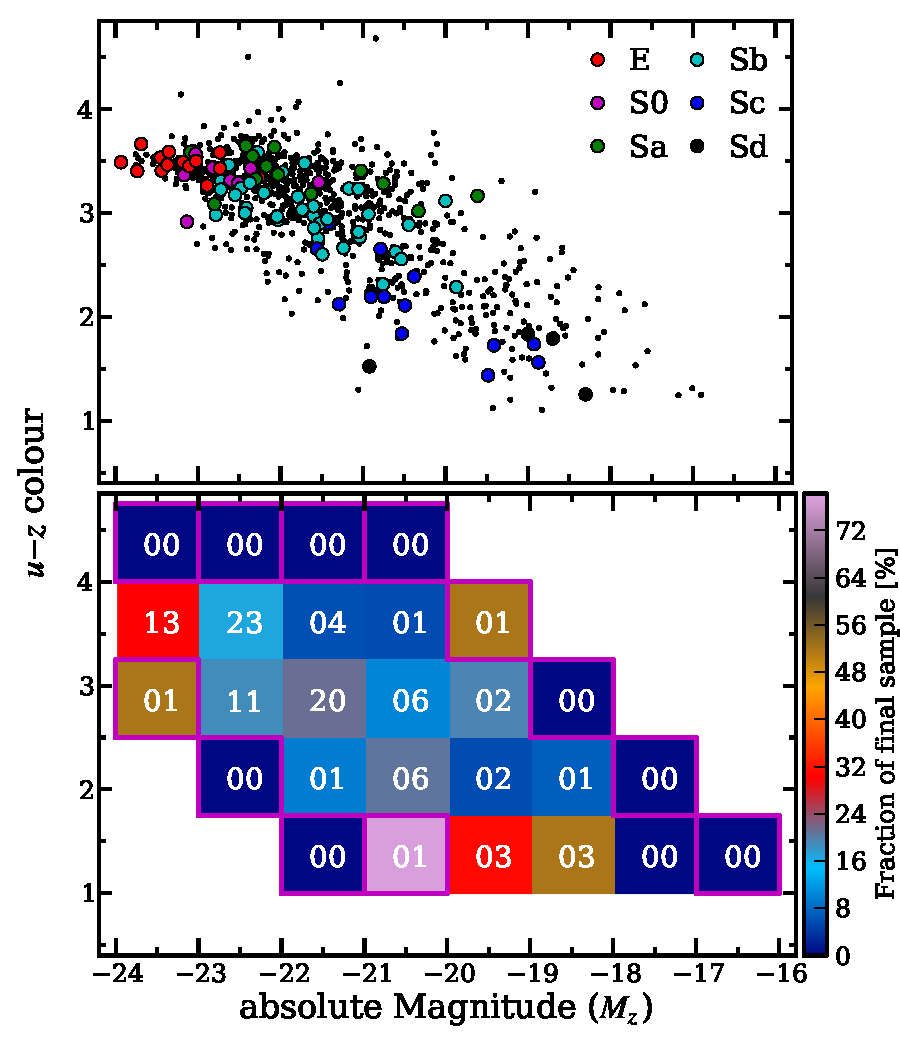
\includegraphics[height=0.5\textwidth]{figuras/figHusemann2013Fig2.pdf}
    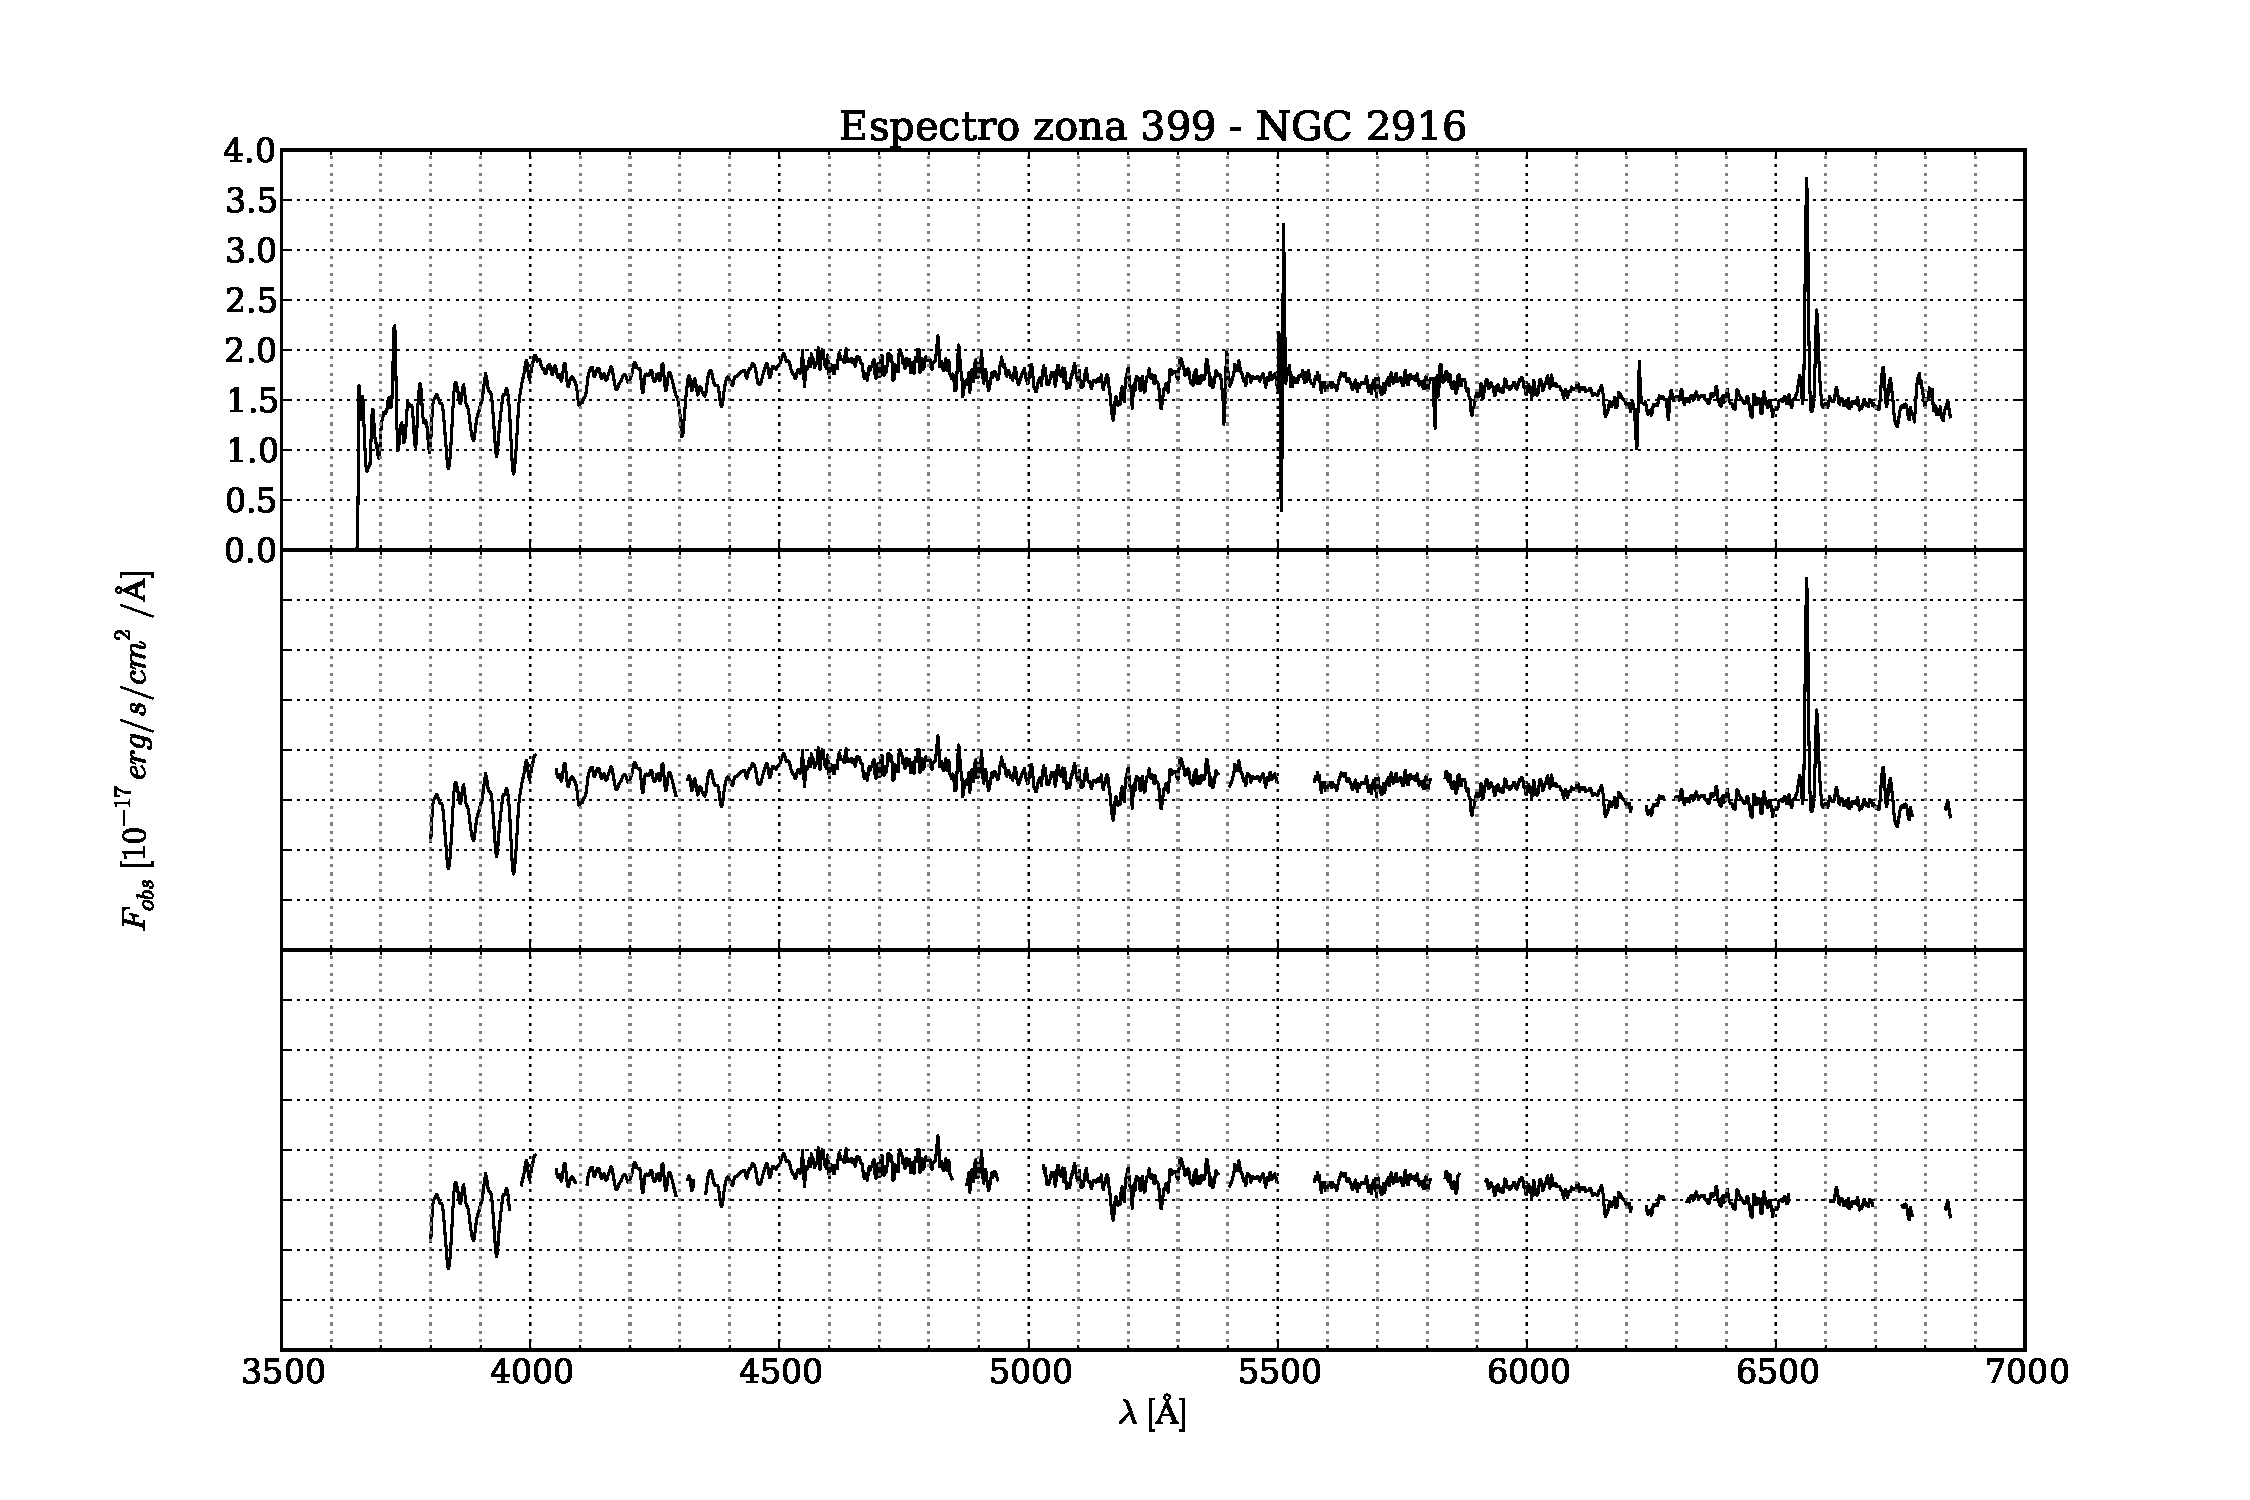
\includegraphics[width=1.0\textwidth]{figuras/K0277-constant_inital_mask-399.pdf}
    \caption[Exemplo de máscaras em um espectro do cubo de dados.]
    {Espectro da zona 399 da galáxia NGC 2916 (CALIFA 277). Acima está o espectro completo. No segundo vemos o espectro
    com linhas telúricas e bad-pixels removidos, além do limite de intervalo em comprimendo de onda de $3800$ a $6850$
    \AA. No espectro mais abaixo, além das partes removidas no segundo, estão foram removidas também as mesmas linhas de
    emissão mascaradas na síntese de populações estelares.}
    \label{fig:UsoPCA:checkmask}
\end{figure}

\begin{figure}
    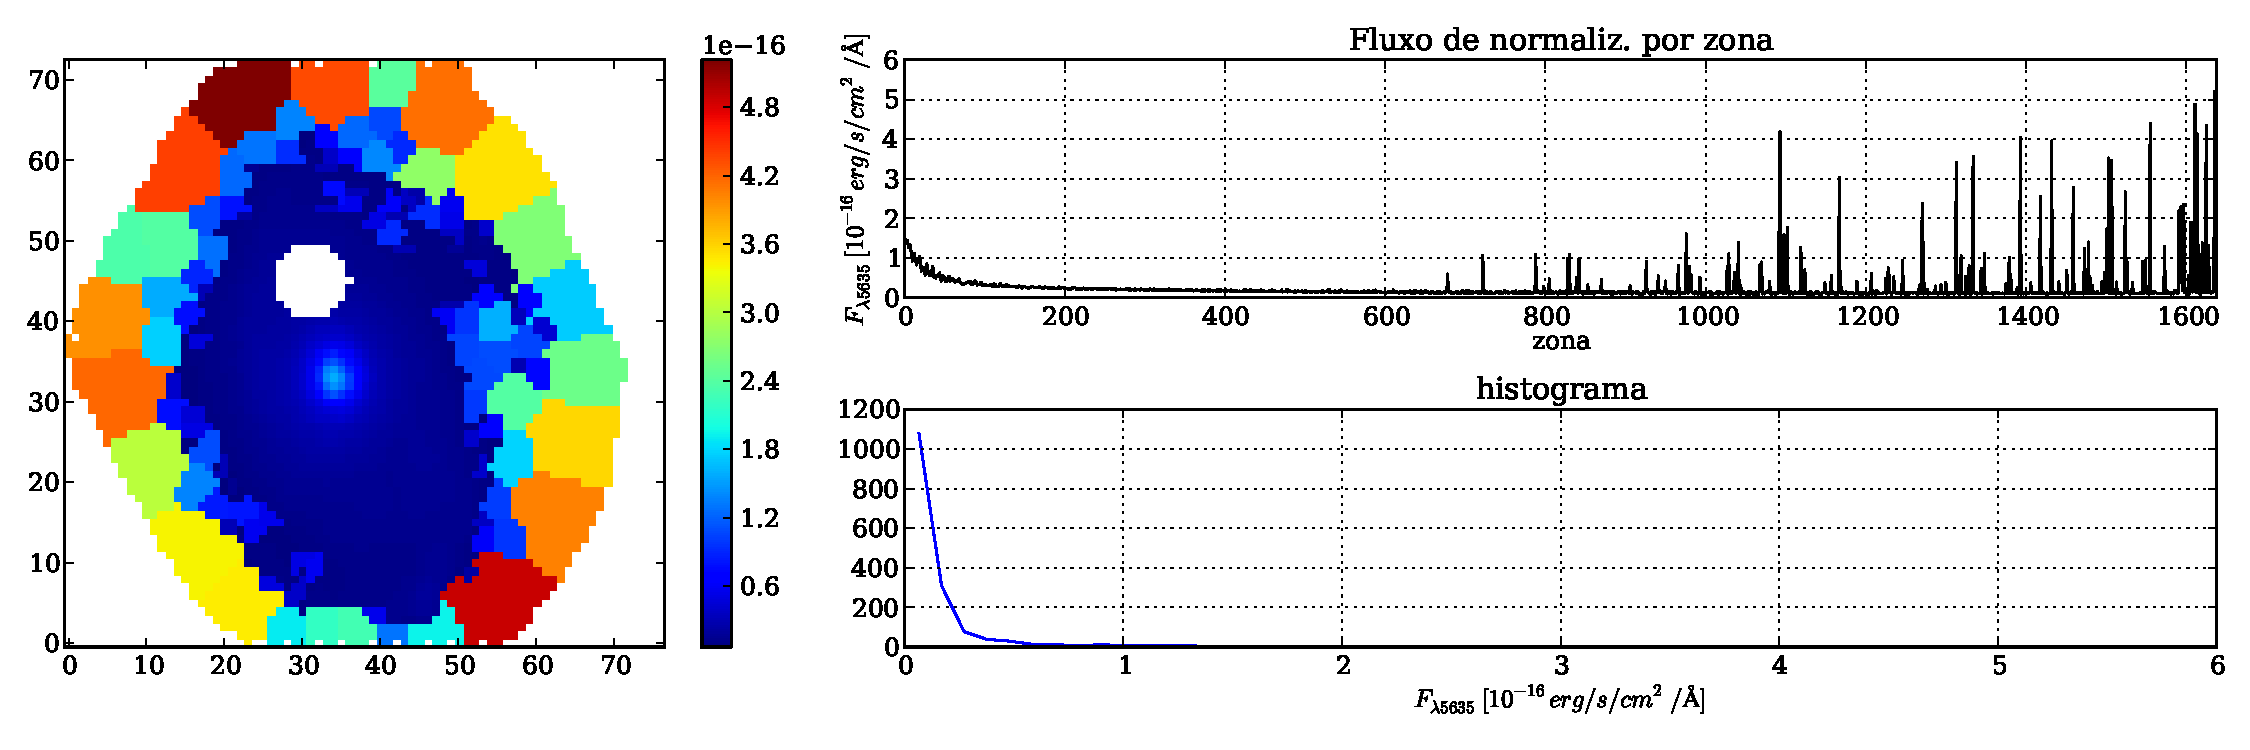
\includegraphics[width=1.\textwidth]{figuras/K0277-fobs_norm.pdf}
    \caption[Fluxos de normalização para cada zona da galáxia K0277.]
    {A imagem à esquerda e a superior direita, mostram o fluxo usado para a normalização de cada espectro em
    cada pixel (à esquerda) ou zona (superior direita). Na imagem inferior direita temos um histograma para valores do
    fluxo de normalização.}
    \label{fig:UsoPCA:K277fobsnorm}
\end{figure}

\subsection{Normalização}
\label{sec	:UsoPCA:PCAlidades:norm}

Imagine uma galáxia composta inteiramente pela mesma população estelar, em repouso, distribuídas da mesma maneira no
espaço. Ou seja, em qualquer ponto da galáxia o espectro é o mesmo. Um PCA nessa galáxia hipotética nos mostraria apenas
uma componente relevante. Adicione então a essa galáxia uma função de densidade de massa em função do raio, permitindo
que de uma posição para outra a quantidade dessa determinada população se altera (mudando o brilho superficial da
região). Uma componente nova irá surgir na sua análise PCA, mostrando que existe uma variância agora numa componente de
escala (amplitude) nos espectros. Mas o que essa componente de escala nos diz sobre a física da população estelar
existente? Essa componente seria um disperdício de variância para uma análise de populações estelares de uma galáxia.

No caso do CALIFA, o cubo de espectros inclui um {\em FoV} que abrange praticamente toda a galáxia. Isso gera uma
variância indevida entres as zonas devido a luminosidade mais intensa nas zonas centrais da galáxia em comparação com as
mais afastadas. Indevidas pois não trazem informação nova para a nossa análise, essas diferenças em amplitude não nos
dizem nada sobre as populações estelares. Nas Figuras \ref{fig:UsoPCA:K277tomofobs} e \ref{fig:UsoPCA:K277tomofobsnorm}
vemos os quatro primeiros tomogramas para a galáxia NGC2916 sem e com normalização. Podemos notar que o primeiro
autoespectro (e seu respectivo tomograma) no caso sem normalização mostra exatamente esse fator de escala. A PC1 se
assemelha muito com a média (basta multiplicá-lo por -1). Seu tomograma, que reflete o peso dessa componente pra cada
zona da galáxia, é claramente um fator de escala (que pode ser considerado um fator de brilho). É fácil de notar a
semelhança entre a primeira componente do caso com normalização e a segunda componente do caso sem normalização. Outra
comparação que evidencia esse fator de escala é comparar a PC1 do caso sem normalização com os valores usados para a
normalização dos espectros. Para a galáxia NGC2916 os valores estão na Figura \ref{fig:UsoPCA:K277fobsnorm}. Nossas
análises daqui para frente consideremos que cada espectro do cubo é normalizado pelo seu fluxo em $5635$ \AA.

\begin{figure}
    %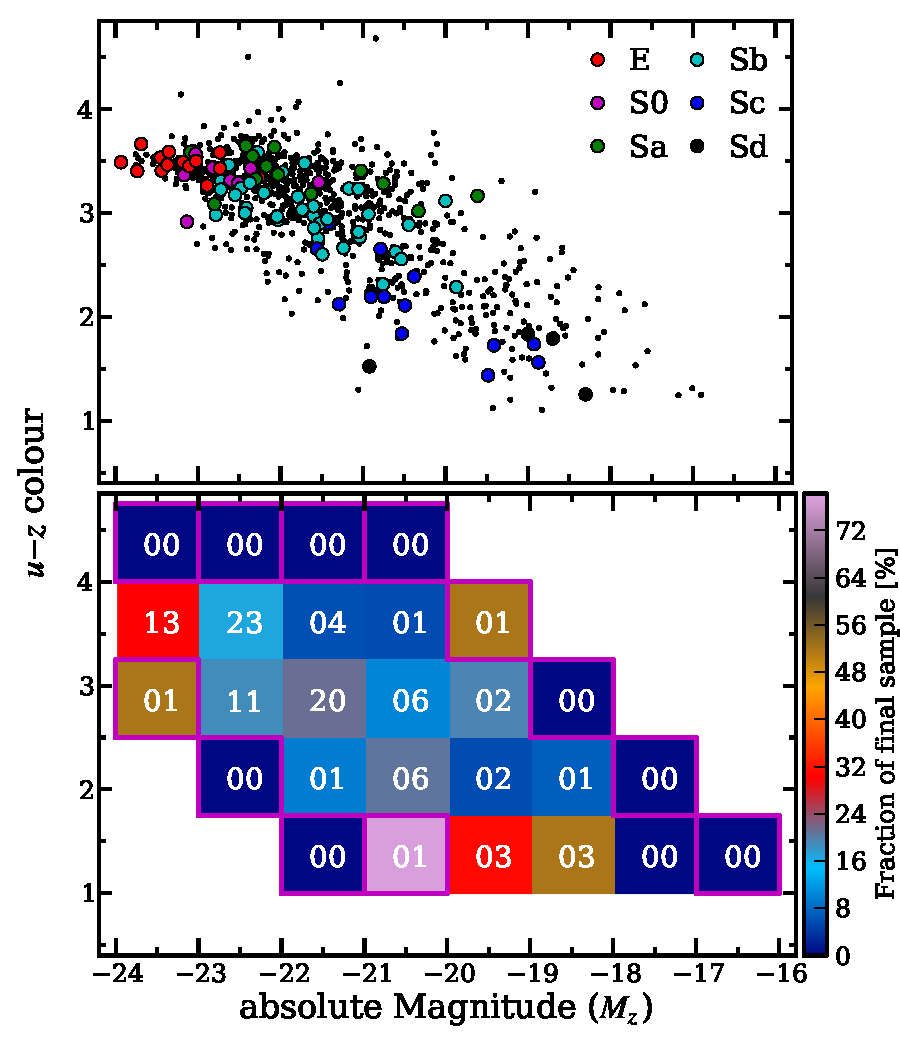
\includegraphics[height=0.5\textwidth]{figuras/figHusemann2013Fig2.pdf}
    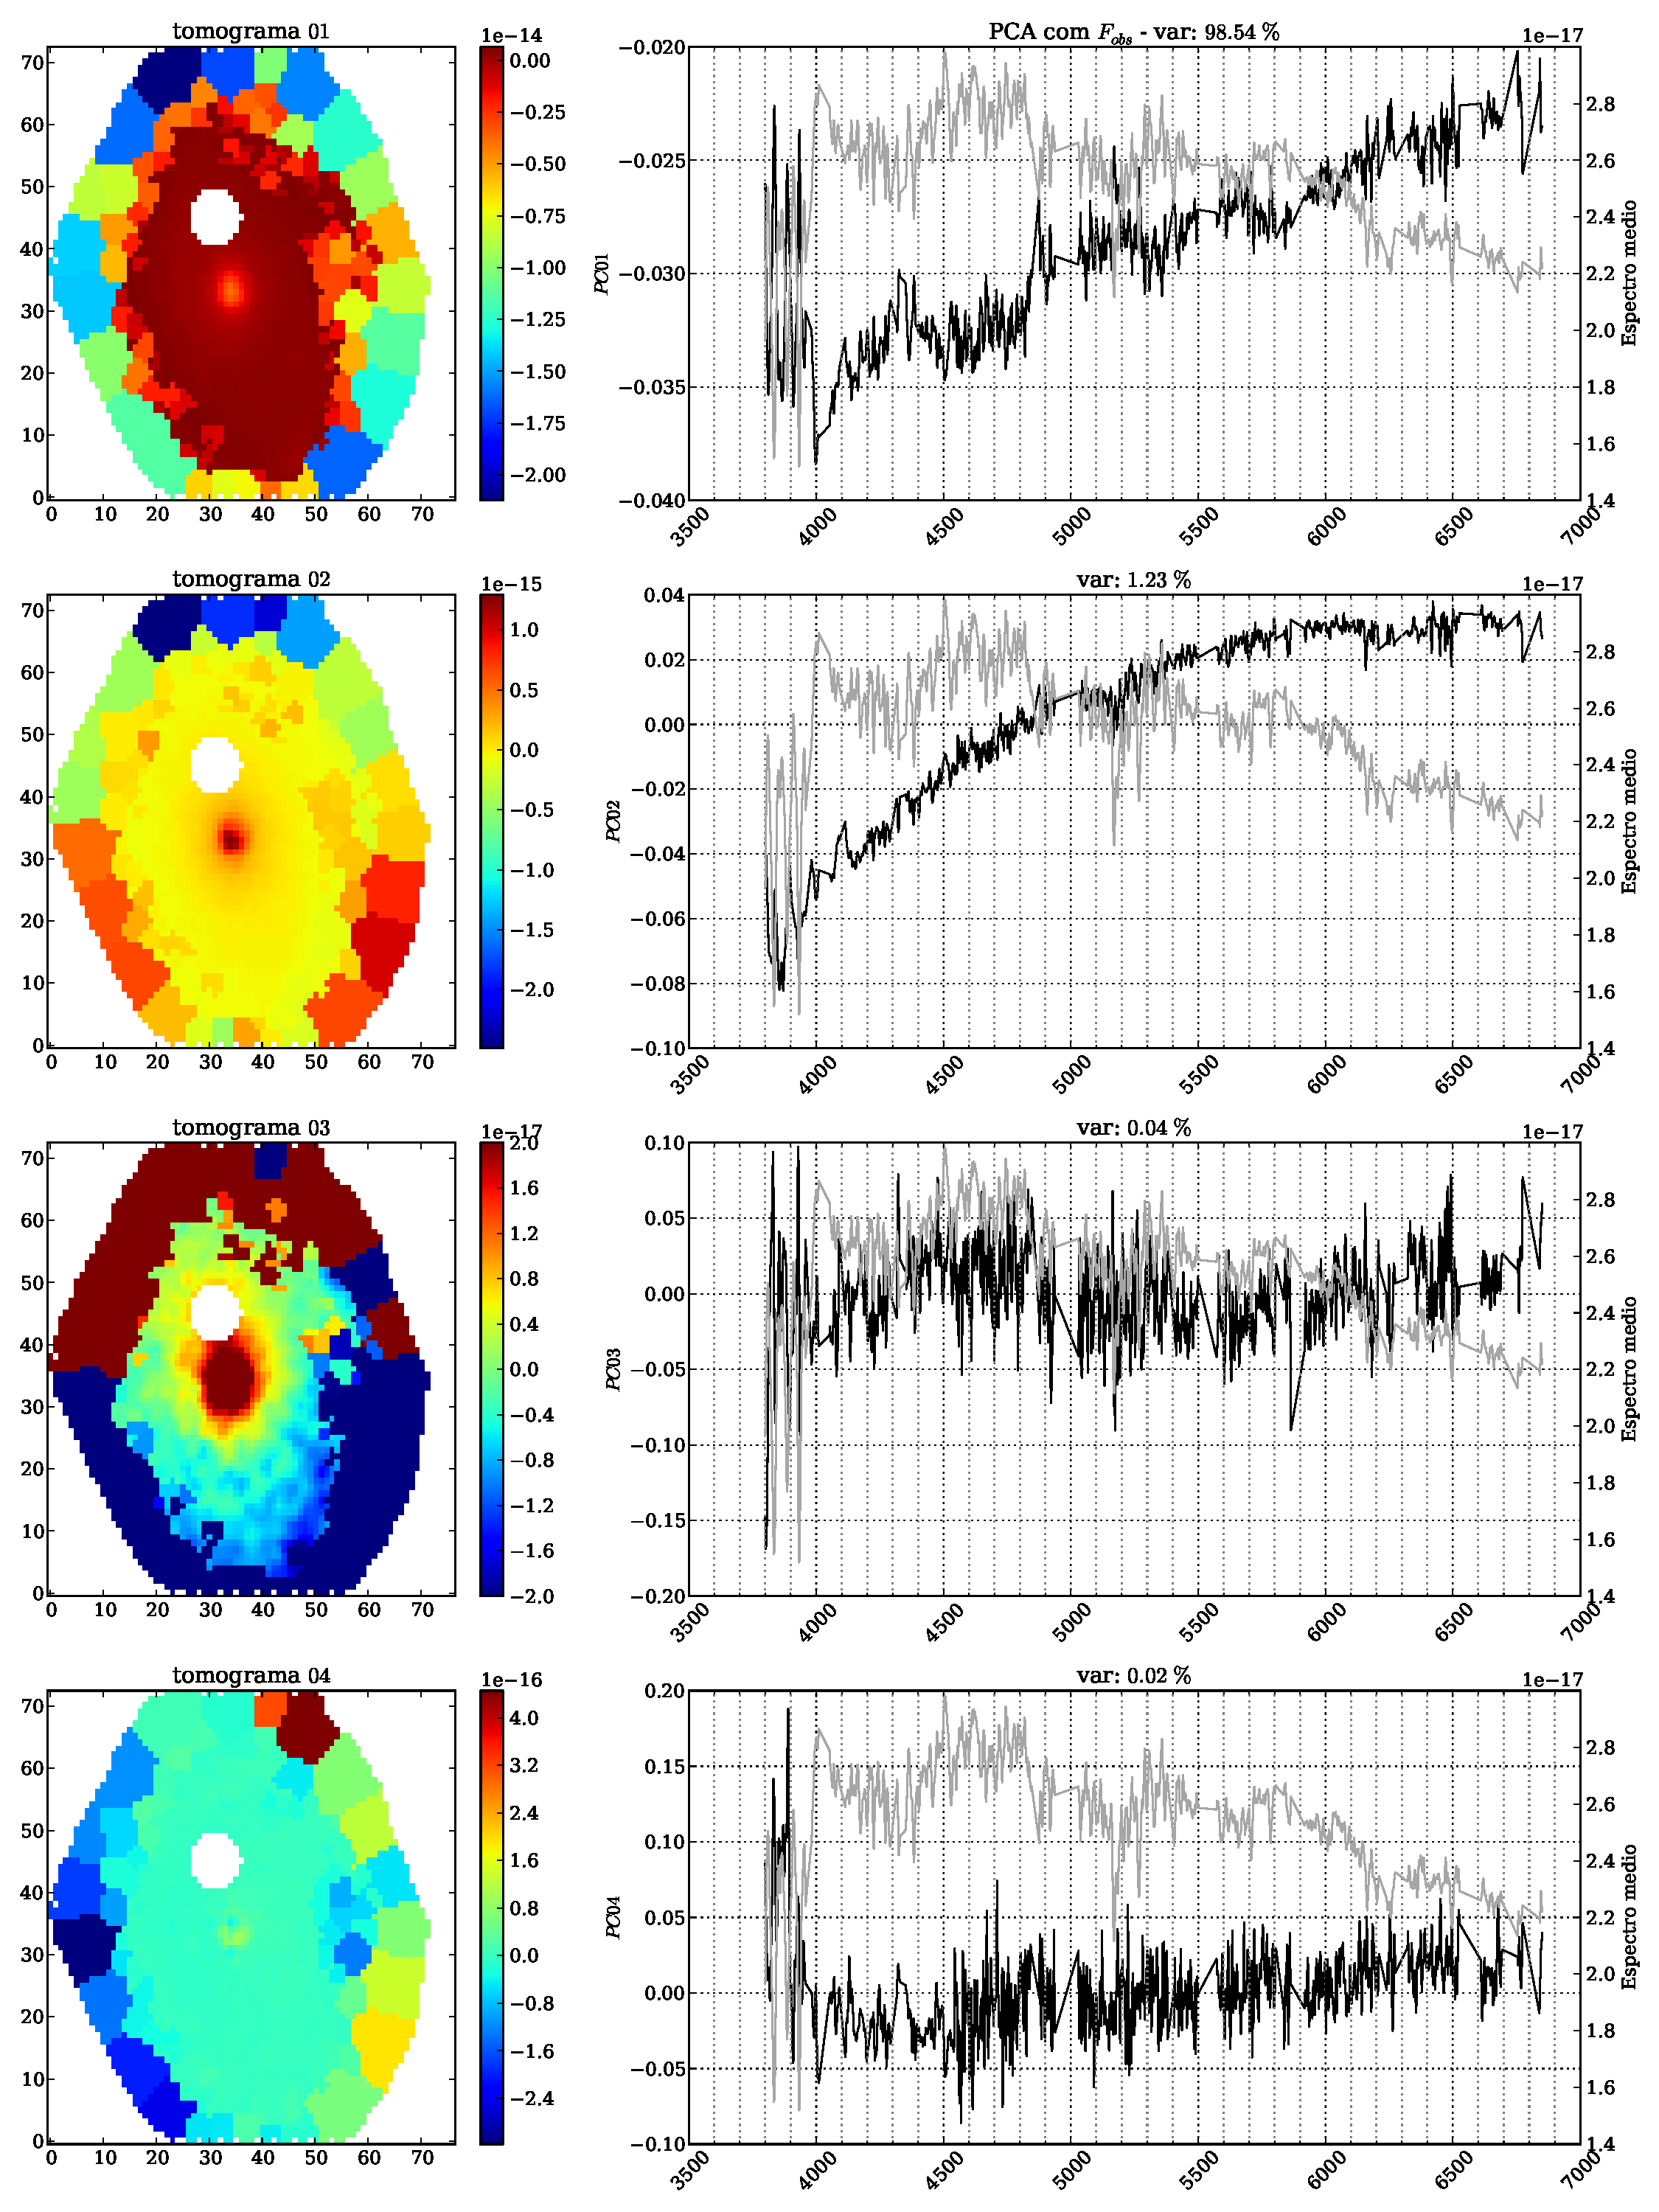
\includegraphics[width=1.\textwidth]{figuras/K0277-tomo1a4.pdf}
    \caption[Tomogramas de 1 a 4 da gal\'axia NGC2916 - sem normaliza\c{c}\~ao.]
    {Quatro primeiros PCs (e seus respectivos tomogramas) do PCA aplicado aos espectros sem normalização da galáxia
    NGC2916.}
    \label{fig:UsoPCA:K277tomofobs}
\end{figure}
\begin{figure}
    %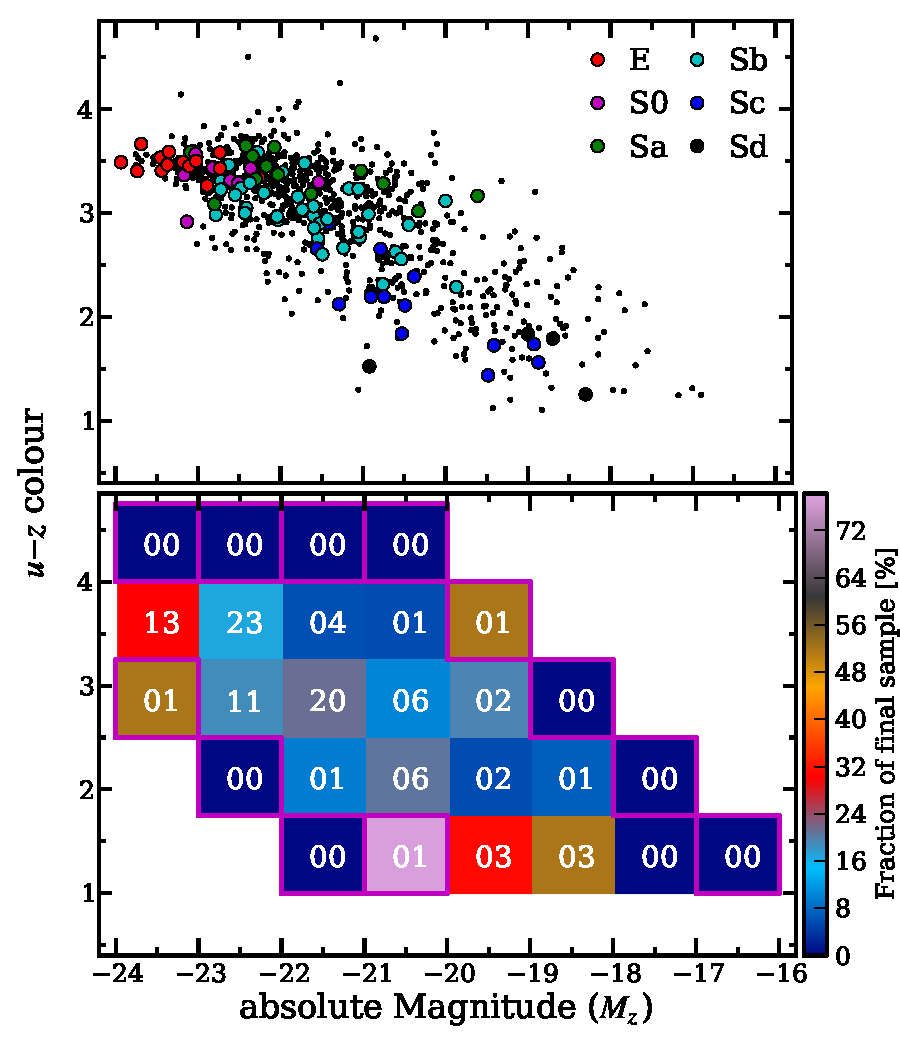
\includegraphics[height=0.5\textwidth]{figuras/figHusemann2013Fig2.pdf}
    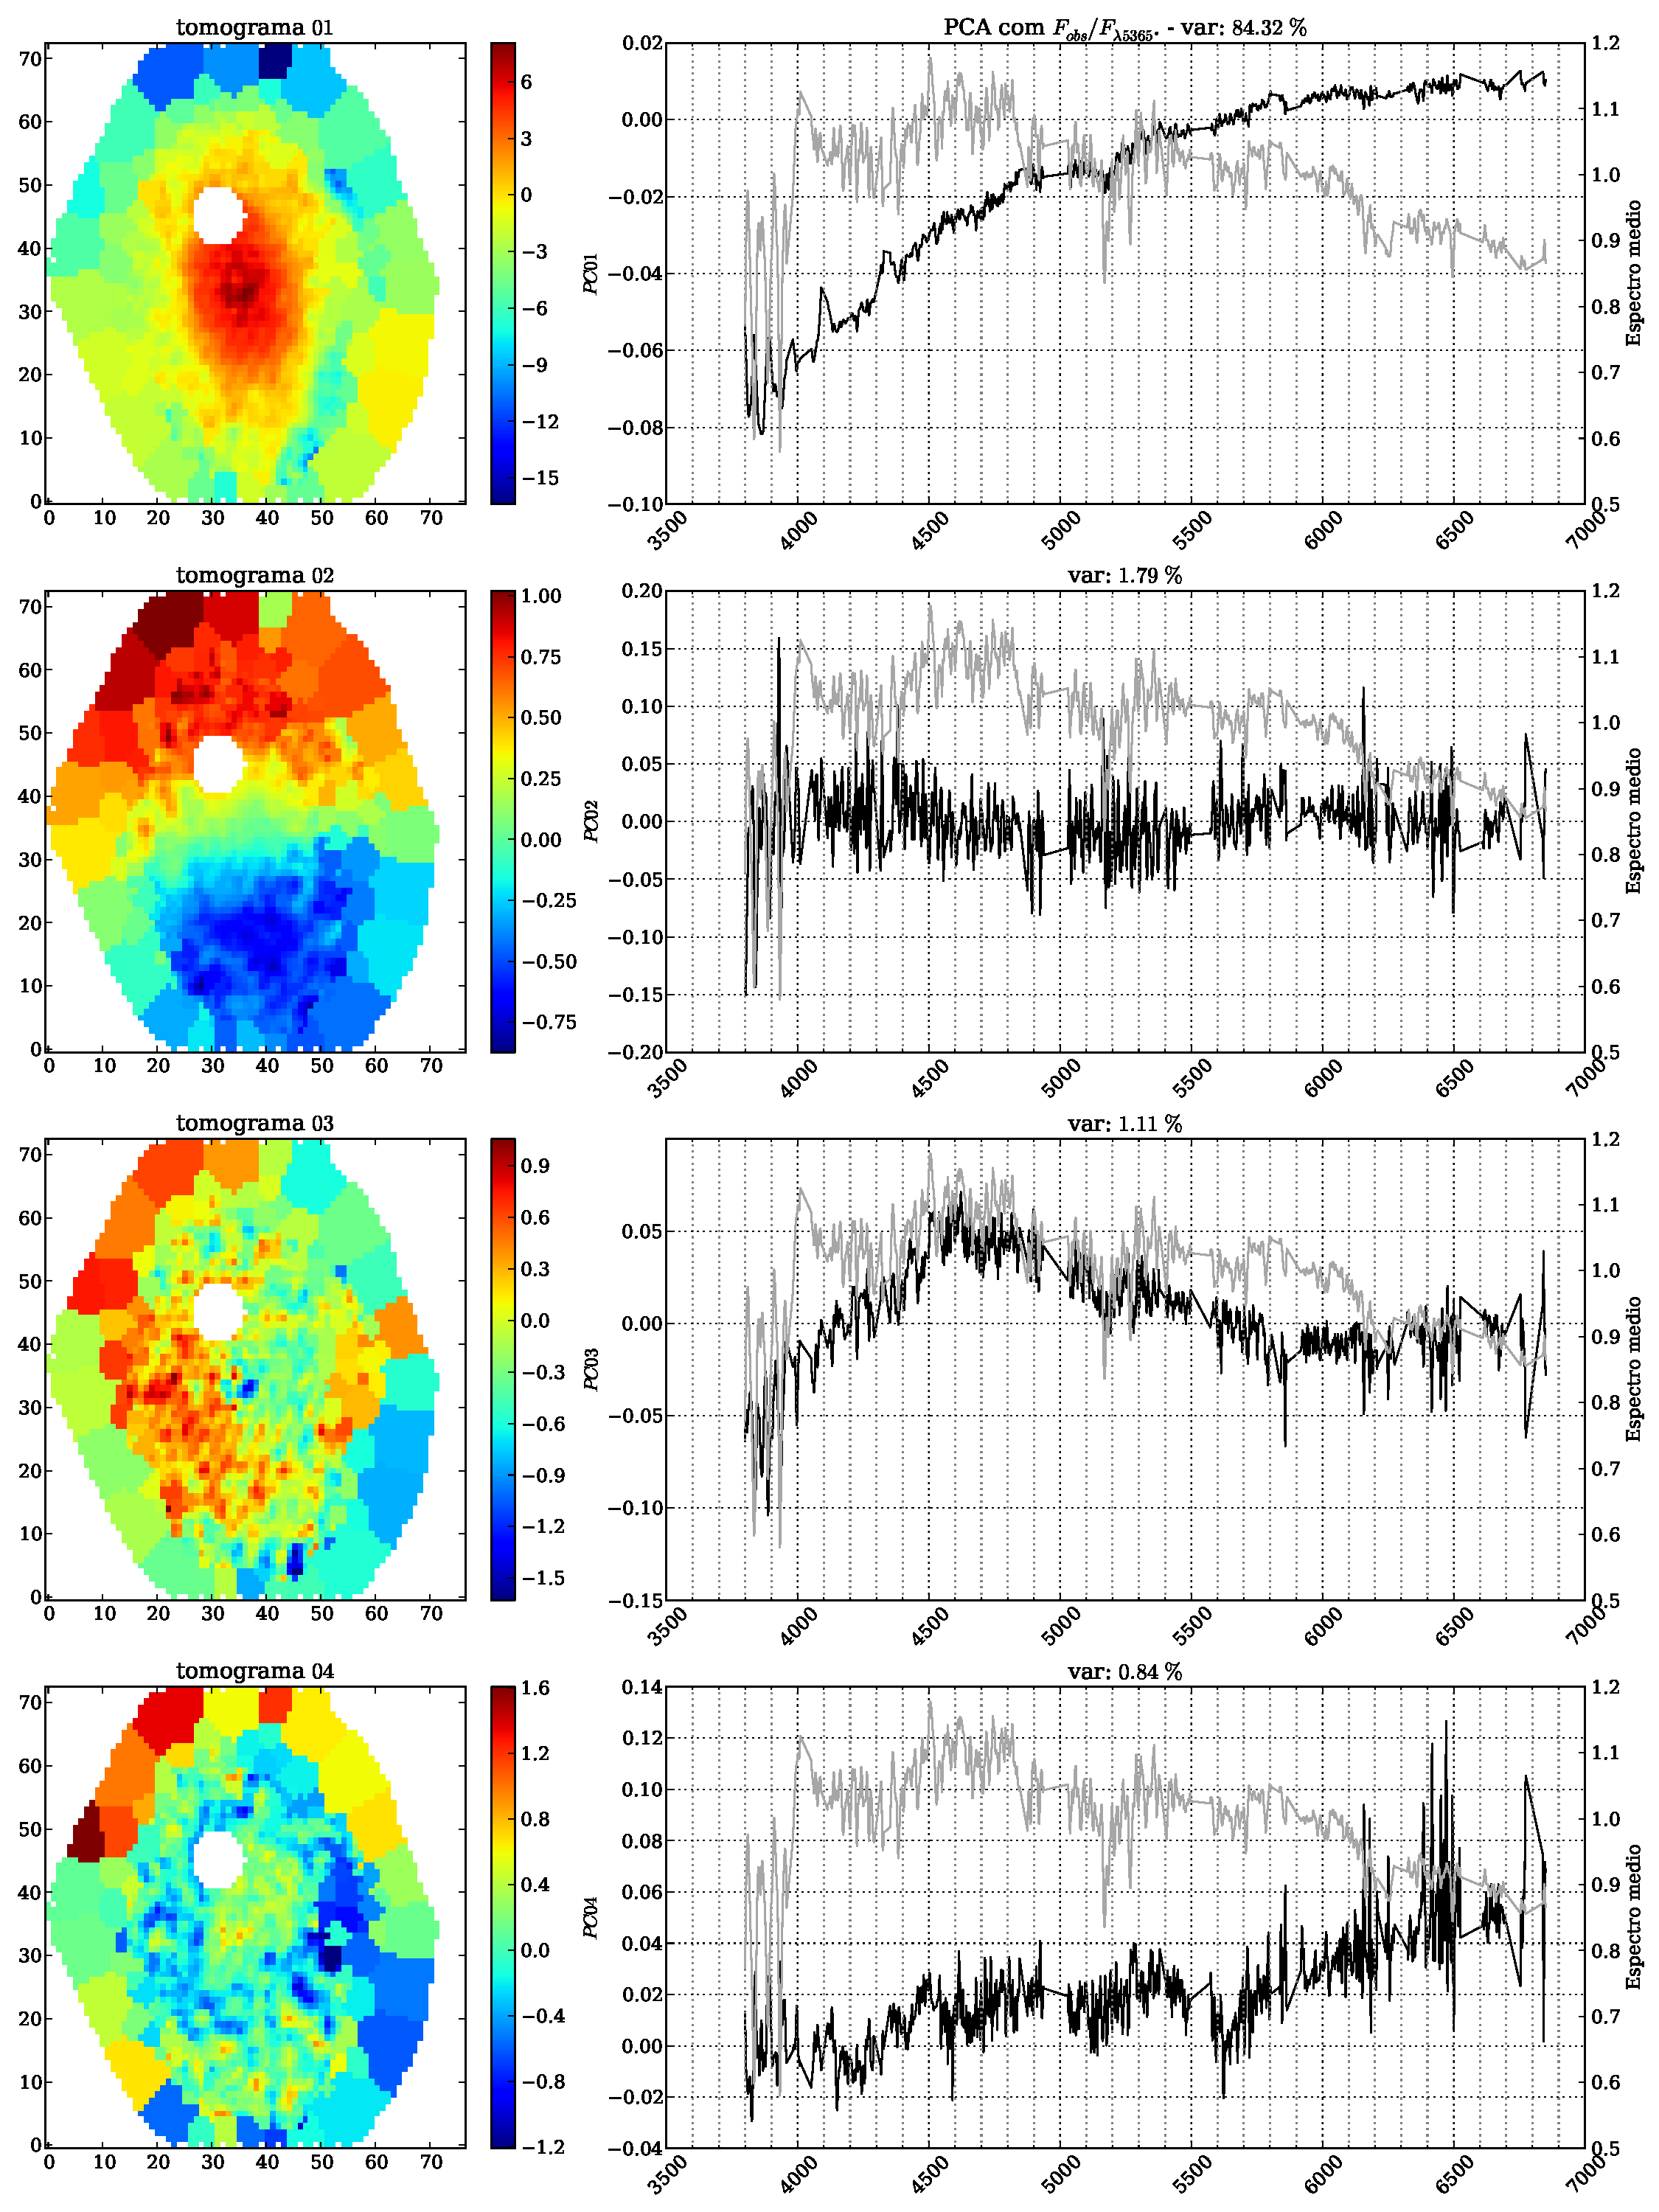
\includegraphics[width=1.\textwidth]{figuras/K0277-tomo1a4-norm.pdf}
    \caption[Tomogramas de 1 a 4 da gal\'axia NGC2916 - com normaliza\c{c}\~ao.]
    {Quatro primeiros PCs (e seus respectivos tomogramas) do PCA aplicado aos espectros com normalização da galáxia
    NGC2916.}
    \label{fig:UsoPCA:K277tomofobsnorm}
\end{figure}

\subsection{Cinemática}
\label{sec:UsoPCA:PCAlidades:cinem}

Usando novamente a ideia da galáxia hipotética com apenas uma população estelar, imagine agora que elas estão
distribuídas uniformemente, mas estão em rotação com a galáxia. Da mesma forma o espectro de todas será igual salvo por
deslocamentos em $\lambda$ no espectro. Esses efeitos cinemáticos não estão nos trazendo informação alguma para o estudo
das populações estelares. Causam um grande disperdício de variâncias, sempre aparecendo nas primeiras PCs. Também é
importante lembrar que existem métodos mais eficazes e direcionados para a determinação de tais propriedades
cinemáticas. Nas galáxias presentes no CALIFA não poderia ser diferente, portanto os espectros aparecem com linhas
deslocadas para o azul ({\em blue-shifted}) ou para o vermelho ({\em red-shifted}) dependendo da velocidade de rotação
projetada. A disperção de velocidades em cada ponto da galáxia também pode causar alargamento ou estreitamento das
linhas.

Podemos ver um padrão bem claro de rotação na PC2 da Figura \ref{fig:UsoPCA:K277tomofobsnorm}. Da mesma forma, na PC3 da
Figura \ref{fig:UsoPCA:K277tomofobs}. Nesta última, fizemos alguns ajustes na saturação das cores de modo que diminuisse
o efeito do fator de escala ainda presente, de modo que ficasse mais evidente o padrão de rotação. É claro que como não
há a normalização, ou seja, ainda há uma mistura de variância pelas intensidades misturado nessa PC, o padrão de rotação
não é tão evidente, diferentemente da PC2 do PCA com normalização.

\subsection{Linhas de emissão e intervalos específicos em comprimento de onda}
\label{sec:UsoPCA:PCAlidades:emlin}

Podemos também executar o PCA apenas em intervalos específicos do espectro. Isso pode ser feito de várias formas, por
exemplo utilizando todos os pontos do(s) intervalo(s) em $\lambda$, ou utilizando apenas o fluxo integrado, ou apenas
larguras equivalentes de linhas, ou FWHM das linhas. Um exemplo aplicado é fazer o PCA apenas das regiões que abrangem
$\oIII/\Hbeta$ em conjunto com $\nII/\Halpha$ ou então $\mathrm{H}\delta$ e D$4000$ para estudar a variância espacial
desses ratios.

\section{Comparando as PCs com o \starlight: engenharia reversa}
\label{sec:UsoPCA:EngRev}

Nos espectros, além dos {\em bad pixels} e linhas telúricas, podemos mascarar regiões desnecessárias para determinada
investigação científica. Nosso foco é o estudo das populações estelares, portanto necessitamos que as linhas de emissão,
geralmente associadas ao gás presente nas galáxias \fixme sejam removidas do espectro. Dessa forma podemos fazer
correlações entre os resultados do PCA e as propriedades físicas obtidas pela síntese.Em nossas análises no próximo
capítulo \ref{sec:result} são mascaradas também todas as regiões que são removidas na síntese ($\mathrm{H}\epsilon$: de
$3960$ a $3980$ \AA; $\mathrm{H}\delta$: de $4092$ a $4112$ \AA; $\mathrm{H}\gamma$: de $4330$ a $4350$ \AA; \Hbeta: de
$4848$ a $4874$ \AA; \oIII: de $4940$ a $5028$ \AA; $\mathrm{He\,\textsc{i}}$ e $\mathrm{NaD}$: de $5866$ a $5916$ \AA;
\Halpha e \nII: de $6528$ a $6608$ \AA; $\mathrm{S\,\textsc{ii}}$: de $6696$ a $6752$ \AA). O espectro após todas
máscaras pode ser visto no terceiro espectro (o mais abaixo) da Figura \ref{fig:UsoPCA:checkmask}.

\subsection{Fluxos observados e sintéticos}
\label{sec:UsoPCA:EngRev:ObsvsSyn}

Com o PyCASSO, temos o resultado da síntese de populações estelares já organizado para as galáxias do CALIFA. Com isso
realizamos o PCA no cubo de espectros observados e no de espectros sintéticos, com e sem normalização. A grande
diferença é que nos espectros sintéticos estão contidas apenas as informações sobre populações
estelares\footnote{Suavização, correções por poeira e cinemática também são feitas nos espectros no processo de síntese.
Mais detalhes em \citet{CidFernandes2005}}. Como os espectros sintéticos não possuem as assinaturas dos equipamentos
observacionais, de todo o processo de redução e afins, quando analisadas pela técnica de PCA vemos que as informações se
condensam em menos PCs, ou seja, o número de PCs relevantes é menor para o caso dos espectros sintéticos. Podemos ver
isso comparando os dois {/em scree tests} na Figura \fixme. 

Caso as grandezas físicas analisadas em uma galáxia fossem
não-correlacionadas seria muito mais fácil fazer uma comparação entre PCs e grandezas físicas, mas geralmente não é o
que ocorre. A forma que temos para recolher informações de galáxias é ou com imagens ou com espectros. E, em ambas
formas, diferentes efeitos físicos causam efeitos semelhantes nas cores (imagem) ou nos espectros. Esses efeitos são
extremamente correlacionados e a muito tenta-se descorrelacioná-los \ojo \citneed \textcolor{red}{Gostaria de adicionar
aqui algumas referências como alguns dos papers do SEAGal/Starlight que fala sobre as degenerescencias de idade e
metalicidade e algumas outras grandezas correlacionadas. Coloquei essa parte aqui pensando naquela crítica que o cara me
fez lá no México sobre as grandezas em astrofísica serem extremamente correlacionadas.}.

\ldots \dots \ldots \ldots

\textcolor{red}{DAQUI PRA BAIXO AINDA É O ESQUELETO}
\ojo A Filosofia desse capítulo é aprender/testar como operar o PCA para que ele
reflita isso ou aquilo... descrevemos uma série de experimentos nesse sentido.

Preprocessamentos e diferentes tipos de PCAs com ou sem linhas, diferentes
faixas espectrais, com dados normalizados ou não. (importante!!!)

Vamos nos limitar a no-emission lines analysis, descrever a máscara de linhas de
emissão, etc. Isso para facilitar a coisa e pq queremos correlar o resultado do
PCA com os dados do Starlight (PyCASSO).

Simulações para ajudar a decifrar os resultador, população jovem + velha +
modelo de distribuição espacial - ver efeitos de estratégias de
preprocessamento.

Correlacionando os resultados do PCA com as propriedades do starlight (tipo de
engenharia reversa)

Linhas telúricas - remover ou não... bad pixels... mascarar ou não linhas de
emissão